\appendix

\section{The Web Platform}

\subsection{1-mathml-in-html}

The demo shows that MathML integrates well inside HTML page. It can easily be 
styled like the text ({\tt font-family: Neo Euler, font-size: 64pt, color: white}), 
scales according to the font-size and has good vertical alignment with respect 
to the surrounding text. 

\href{http://fred-wang.github.io/MathUI2014/demos/1-mathml-in-html.html}{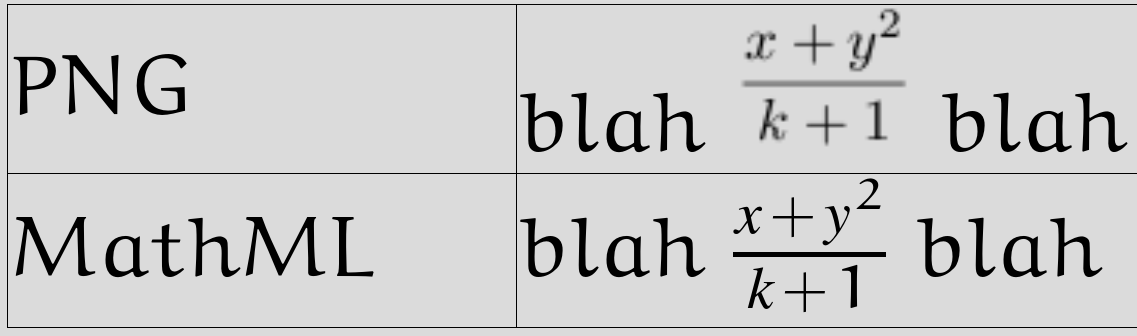
\includegraphics[width=\textwidth]{screenshots/1-mathml-in-html}}

\subsection{2-mathml-in-svg}

The demo is an SVG image with MathML formulas embedded via the
{\tt <foreignObject>} element.

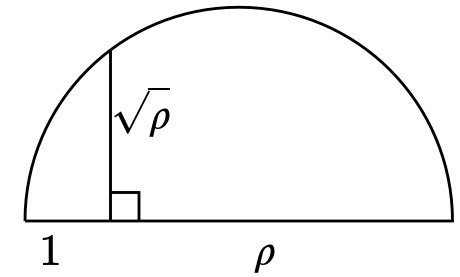
\includegraphics{screenshots/2-mathml-in-svg}

\subsection{3-mathml-javascript}

The demo shows how Javascript can be used to produce interactive documents.
Clicking on the button will successively highlight different terms of Sarrus'
rule. Below is a screenshot of the three first steps.

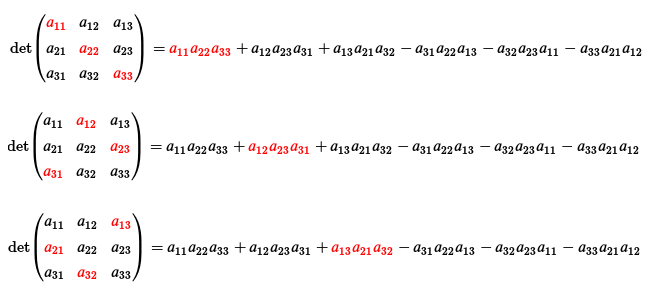
\includegraphics{screenshots/3-mathml-javascript}

\subsection{5-canvas}

The graphs in this demo are drawn using canvas. They are updated automatically
when you modify the current frequency.

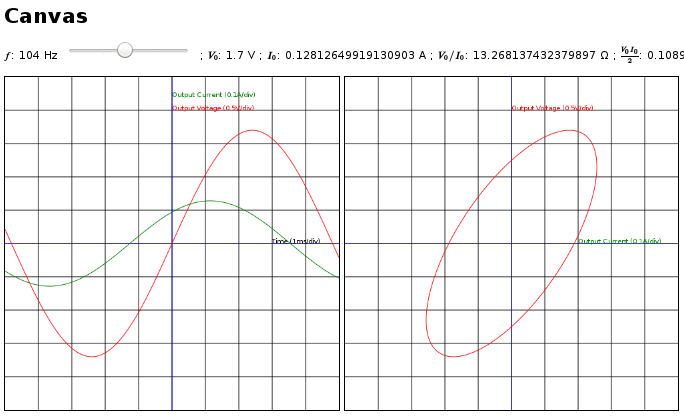
\includegraphics{screenshots/5-canvas}

\subsection{4-mathml-fonts}

Below are screenshots of the page with different fonts in Firefox 31 for Linux.
This is simply achieved by
using the classical CSS rule {\tt font-family} with optional {\tt @font-face}
rules to define a fallback with Web fonts. Gecko 31 is required to get the
different fonts used for the drawing of operators (e.g. the integral and
sum symbols). Other features of the OpenType MATH table (e.g. gaps or
linethickness) are not implemented yet in this version.

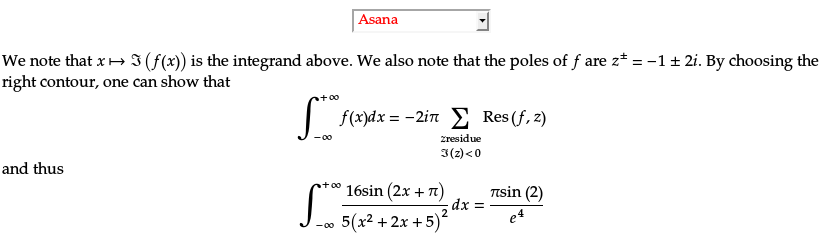
\includegraphics[width=\textwidth]{screenshots/4-mathml-fonts-asana}

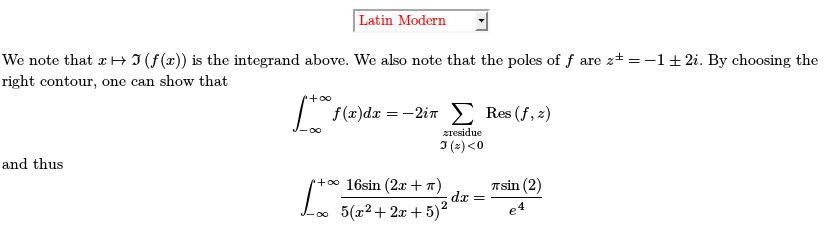
\includegraphics[width=\textwidth]{screenshots/4-mathml-fonts-latin-modern}

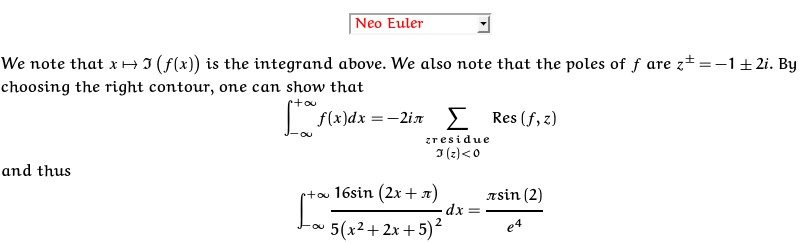
\includegraphics[width=\textwidth]{screenshots/4-mathml-fonts-neo-euler}

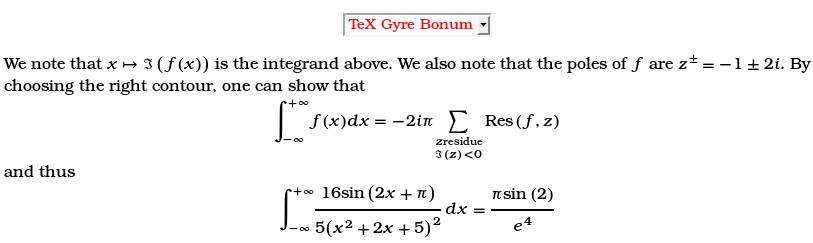
\includegraphics[width=\textwidth]{screenshots/4-mathml-fonts-tex-gyre-bonum}

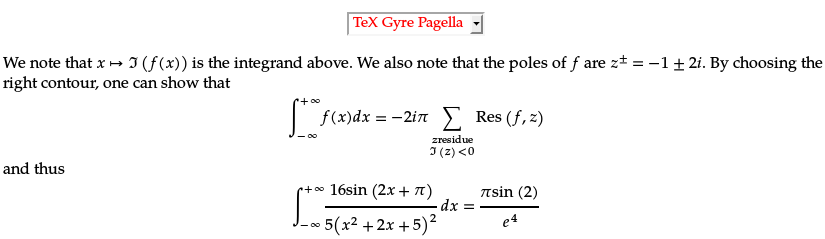
\includegraphics[width=\textwidth]{screenshots/4-mathml-fonts-tex-gyre-pagella}

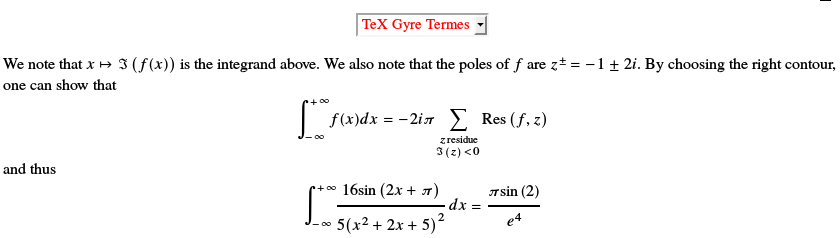
\includegraphics[width=\textwidth]{screenshots/4-mathml-fonts-tex-gyre-termes}

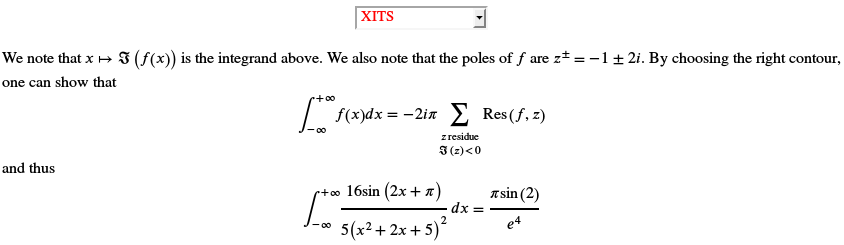
\includegraphics[width=\textwidth]{screenshots/4-mathml-fonts-xits}

\subsection{6-mathml-in-webgl}

The 3D schema in this demo is drawn using WebGL and has MathML formulas
included inside.

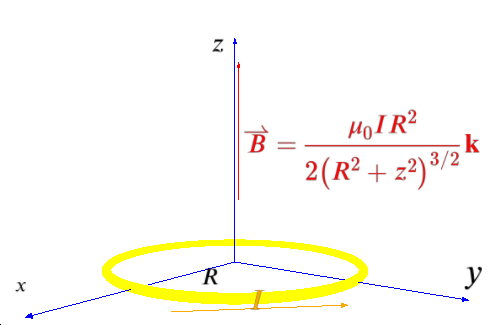
\includegraphics{screenshots/6-mathml-in-webgl-1}

You can interactively move and rotate the schema using the mouse. Here is the
same schema seen from above, which more clearly shows the circular loop and it
radius.

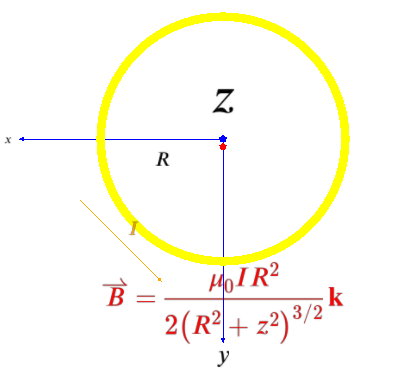
\includegraphics{screenshots/6-mathml-in-webgl-2}

\subsection{7-web-component}

The page contains the following code:

\begin{verbatim}
  <x-tex display="block">\Gamma(t) =
    \lim_{n \to \infty} \frac{n! \; n^t}{t \; (t+1)\cdots(t+n)} =
    \frac{1}{t} \prod_{n=1}^\infty \frac{\left(1+\frac{1}{n}\right)^t}{1+\frac{t}{n}} =
    \frac{e^{-\gamma t}}{t} \prod_{n=1}^\infty \left(1 + \frac{t}{n}\right)^{-1} e^{\frac{t}{n}}
  </x-tex>
\end{verbatim}

which is automatically converted into MathML and renders approximately like
this:

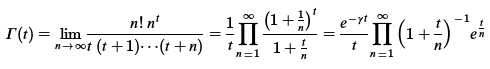
\includegraphics{screenshots/7-web-component}

\section{Firefox OS Apps}

